\documentclass[a4j]{jsarticle}
\usepackage{amsmath,listings}
\usepackage[dvipdfmx]{graphicx}
\newcommand{\figref}[1]{図\ref{#1}}

\title{組込みRTOS向けアプリケーション開発支援ツール\\
TLV(トレース ログ ヴィジュアライザー)\\
フェーズ3 外部仕様書}

\begin{document}
\maketitle
\titlepage

\section*{改訂履歴}
\begin{table}[h]
 \centering
 \begin{tabular}{|c|c|c|c|} \hline
  版番& 日付&    更新内容& 更新者\\ \hline\hline
  1.0 & 09/1/30 & 新規作成& 水野\\ \hline
 \end{tabular}
\end{table}
\clearpage

\tableofcontents
\clearpage

\section{はじめに}
\subsection{本書の目的}
本書の目的は、文部科学省先導的ITスペシャリスト育成推進プログラム「OJLによる最先端技術適応能力を持つIT人材育成拠点の形成」プロジェクトにおける、OJL科目ソフトウェア工学実践研究の研究テーマである「組込みRTOS向けアプリケーション開発支援ツールの開発」に対して、その開発するソフトウェアに対する外部仕様を記述することである。

本書は特に、フェーズ3における外部仕様、つまり要求の詳細な実現方法についての記述を行う。

\subsection{本書の適用範囲}
本書は、組込みMPRTOS向けアプリケーション開発支援ツールの開発プロジェクト
(以下本プロジェクト)におけるフェーズ3に対する詳細な外部仕様を記述する.

\subsection{用語の定義/略語の説明}

\begin{table}[h]
 \centering
 \caption{用語定義}
 \begin{tabular}{|p{8em}|p{36em}|} \hline
  用語・略語& 定義・説明\\ \hline \hline
  TLV& Trace Log Visualizer\\ \hline
  MPRTOS& マルチプロセッサ対応リアルタイムオペレーティングシステム\\
  \hline
  トレースログファイル&
      RTOSのトレースログ機能を用いて出力したトレースログや、
      シミュレータなどが出力するトレースログをファイルにしたもの\\
  \hline
  共通形式トレースログファイル&
      本ソフトウェアが扱うことの出来る形式をもつトレースログファイル。
      各種トレースログファイルは、この共通形式トレースログファイルに
      変換することにより本ソフトウェアで扱うことが出来るようになる。 \\
  \hline
  表示オブジェクト&
      可視化表示する対象\\
  \hline
  表示エリア&
      可視化表示する領域\\
  \hline
  ロード &
  ある時間に実行可能状態のタスクの個数 \\
  \hline
  ロードアベレージ(CPU使用率) &
  ある期間の実行可能状態のタスクの平均個数。ロードの積分で計算可能。 \\
  \hline
  OS全体のロード・ロードアベレージ &
  OS全体で実行可能状態のタククの個数・平均個数 \\
  \hline
  コア別ロード・ロードアベレージ &
  コアごとの実行可能状態のタククの個数・平均個数 \\
  \hline
  優先度別ロード・ロードアベレージ &
  優先度ごとの実行可能状態のタククの個数・平均個数 \\
  \\
  \hline
 \end{tabular}
\end{table}

\subsection{概要}
本書では、組込みMPRTOS向けアプリケーション開発支援ツールの
ソフトウェアの外部仕様を記述する。
本書では、主にフェーズ3で追加する機能の実現方法について記述する。

\clearpage
\section{概要説明}
\subsection{フェーズ3におけるソフトウェアの概要}
開発対象のソフトウェア(以下、本ソフトウェア)は、
組込みRTOS上のアプリケーションの実行時トレースログを解析し、
可視化表示する機能を提供する。

フェーズ2では、共通形式トレースログへの変換やルールファイルによる
可視化表示など、拡張性や柔軟性の支柱となる主要機能を実装した。
また、フェーズ1での評価を元に、UIの見直しや操作機能の追加を行った。

フェーズ3では、選択時点におけるCPU使用率の表示機能の設計および、
CPUごとのタスク表示機能を実装する。

\subsection{フェーズ3で追加するソフトウェアの機能}
\subsubsection{CPU使用率の表示}

\begin{enumerate}
\item ログを読み込む
\item OS全体のロード・ロードアベレージを表示する。(\figref{all})
\item ロード・ロードアベレージの横の\fbox{+}がクリックされると、コア別のロード・ロードアベレージを表示する。(\figref{core})
\item コア別のロード・ロードアベレージの横の\fbox{+}がクリックされると、優先度別のロード・ロードアベレージを表示する。
\end{enumerate}

\begin{figure}
\centering
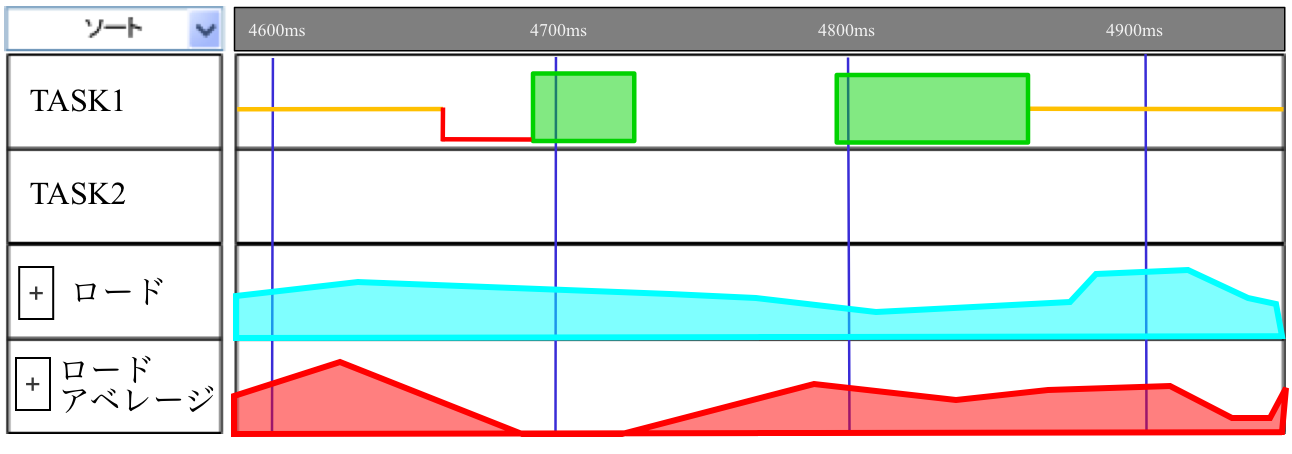
\includegraphics[width=10cm]{all.png}
\caption{OS全体のロード・ロードアベレージ表示}\label{all}
\end{figure}

\begin{figure}
\centering
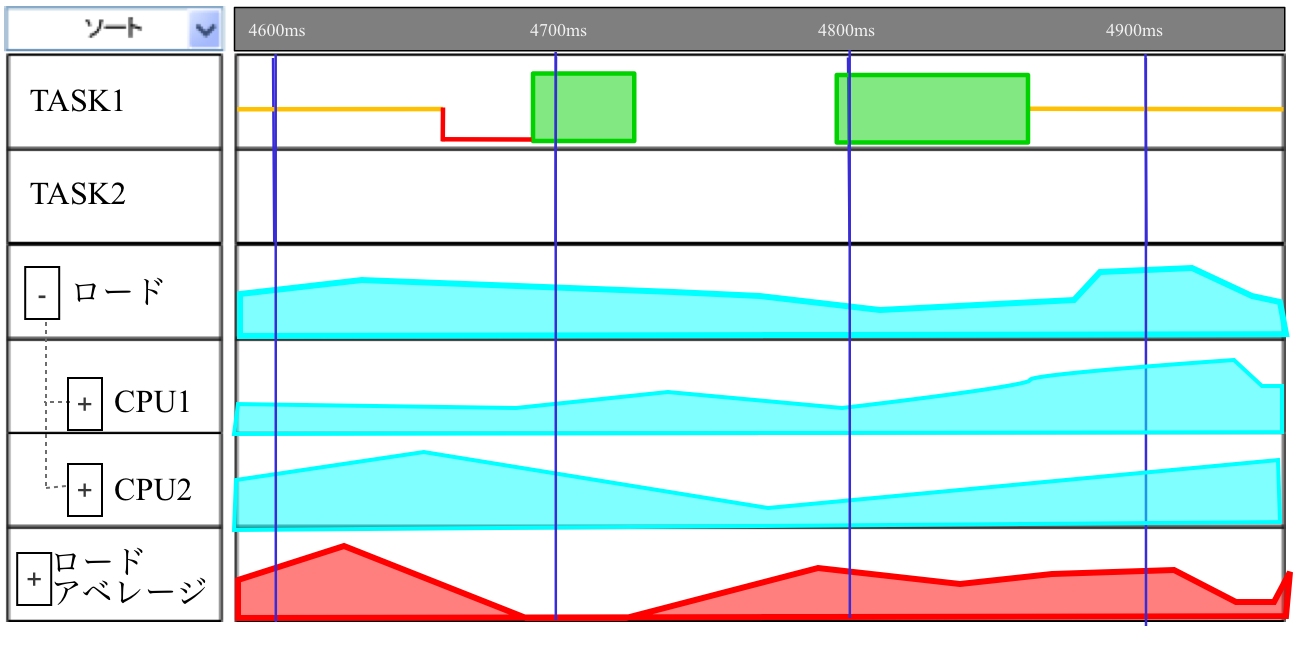
\includegraphics[width=10cm]{core.png}
\caption{コア別のロード・ロードアベレージ表示}\label{core}
\end{figure}

\begin{figure}
\centering
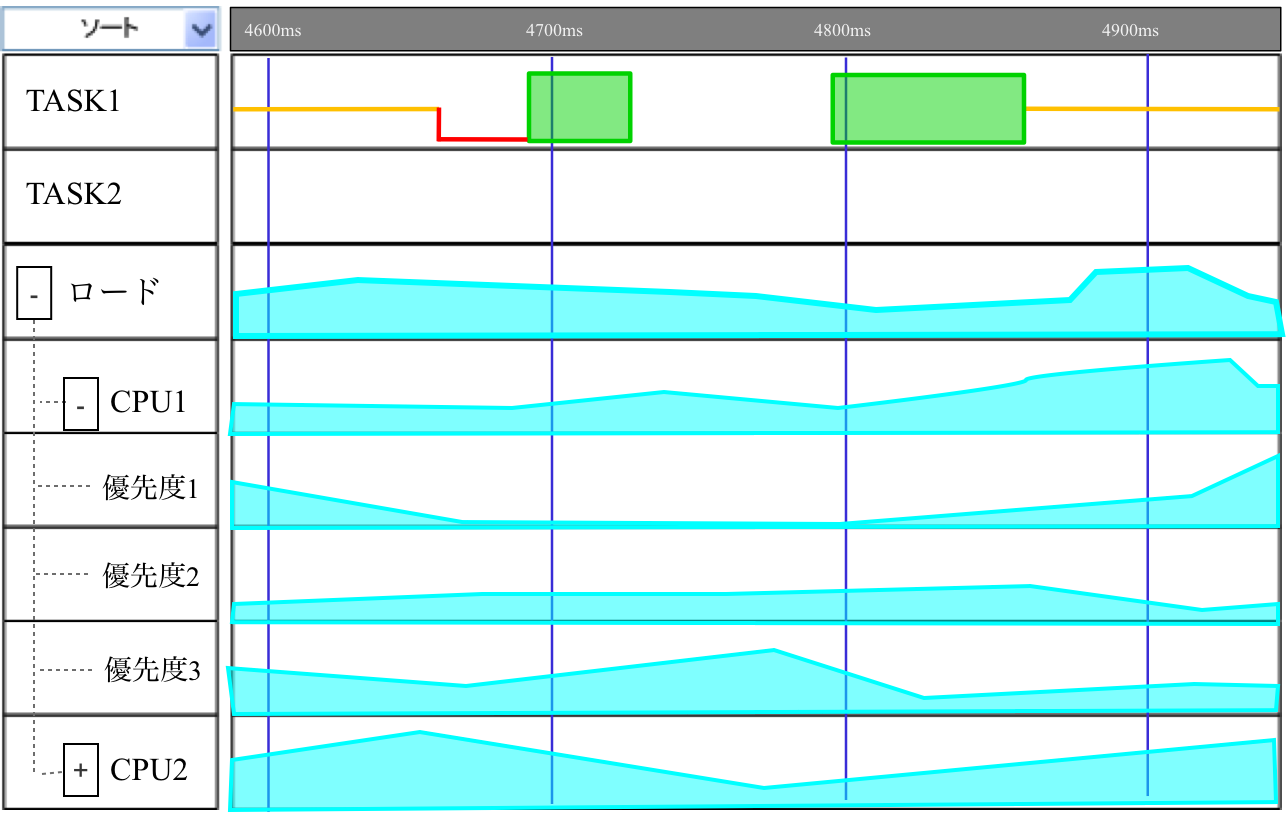
\includegraphics[width=10cm]{pri.png}
\caption{優先度別CPU使用率表示}\label{pri}
\end{figure}

\subsubsection{CPUごとのタスク表示}

\input
\clearpage
\section*{参考文献}

\end{document}
